% Figure 1: Pipeline schematic
\begin{figure}[htbp]
\centering

\includegraphics[width=0.95\textwidth]{figures/fig_schematic.pdf}
\caption{Multi-response LASSO/ridge imputation pipeline. Paired PBMC and sorted
(CD4/CD8/CD14/CD19) RNA-seq from 80 training subjects are used to cluster target
genes into chunks of at most 500 correlated genes via hierarchical clustering on
log$_2$ TPM. For each chunk a penalised multi-response Gaussian model
(\texttt{glmnet}, $\alpha = 1$ for LASSO and $\alpha = 0$ for ridge, five-fold
cross-validated) is fit with all 18{,}871 PBMC genes as predictors and the
chunk's cell-type genes as joint responses, then applied to test PBMCs to
impute cell-type expression.}
\label{fig:schematic}
\end{figure}

% Figure 2: Log2 fold-change attenuation
\begin{figure}[htbp]
\centering
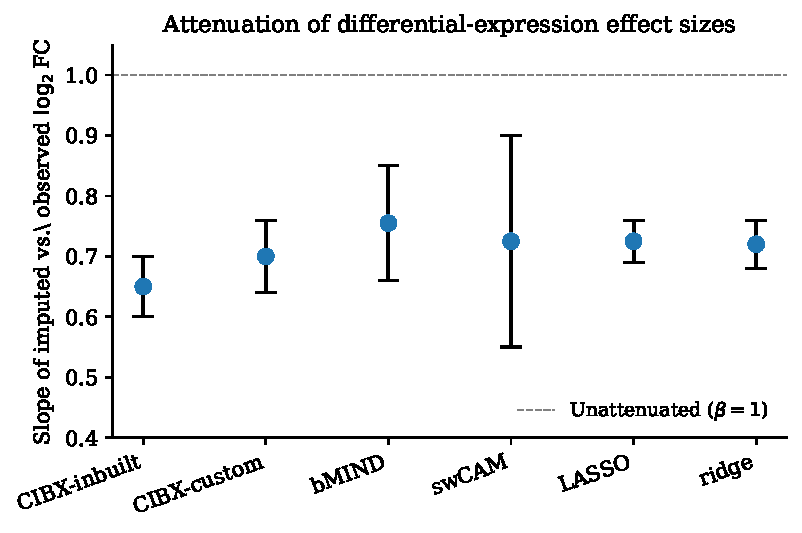
\includegraphics[width=0.75\textwidth]{figures/fig_slopes.pdf}
\caption{Attenuation of imputed $\log_{2}$ fold changes across methods. Ranges
across the four sorted cell types are shown as error bars around the midpoint
for each method: CIBX-inbuilt 0.60--0.70, CIBX-custom 0.64--0.76,
bMIND 0.66--0.85, swCAM 0.55--0.90, LASSO 0.69--0.76, ridge 0.68--0.76. All
methods shrink fold changes relative to the unattenuated ideal ($\beta = 1$,
dashed).}
\label{fig:slopes}
\end{figure}

% Figure 3: Common gene sets
\begin{figure}[htbp]
\centering
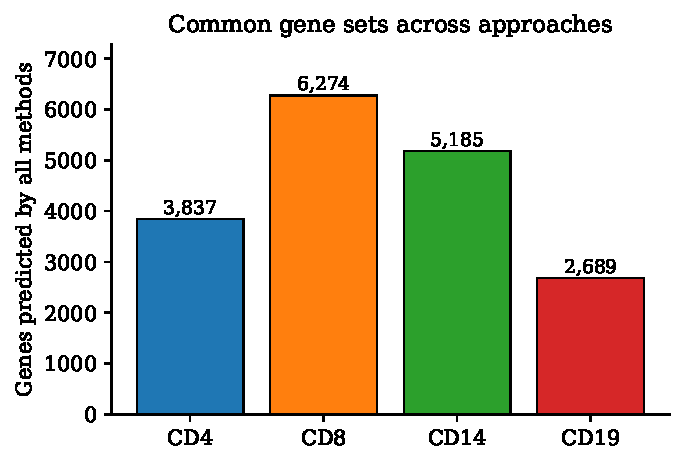
\includegraphics[width=0.6\textwidth]{figures/fig_common_genes.pdf}
\caption{Number of genes predicted by every method, used for the common-gene
sensitivity analysis: CD4, $3{,}837$; CD8, $6{,}274$; CD14, $5{,}185$;
CD19, $2{,}689$.}
\label{fig:common_genes}
\end{figure}

% Figure 4: Computational cost
\begin{figure}[htbp]
\centering
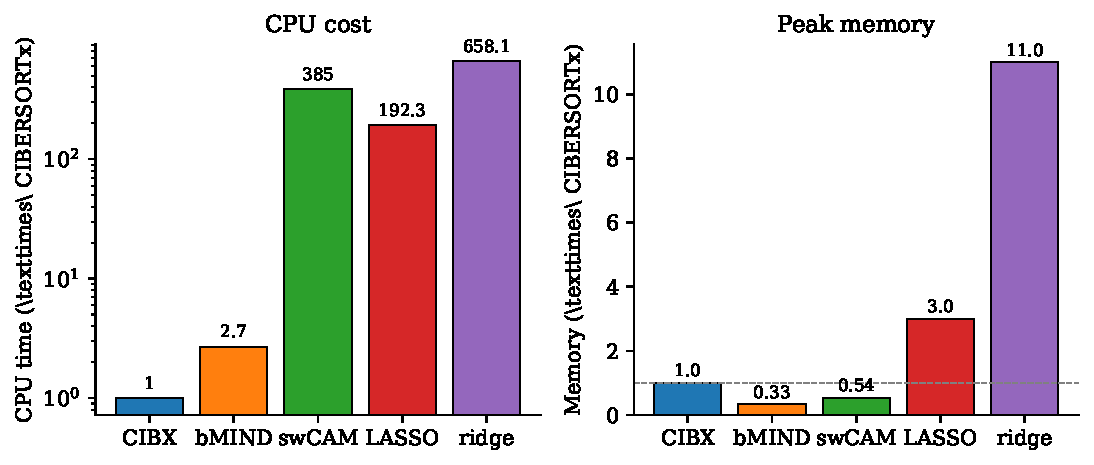
\includegraphics[width=0.9\textwidth]{figures/fig_compute.pdf}
\caption{Computational cost relative to CIBERSORTx. Left: CPU time on a
logarithmic scale; bMIND is $2.7\times$ slower, swCAM $385\times$, LASSO
$192.3\times$, ridge $658.1\times$. Right: peak memory; bMIND uses $33\%$ and
swCAM $54\%$ of CIBERSORTx memory, while LASSO and ridge require up to
$3\times$ and $11\times$, respectively.}
\label{fig:compute}
\end{figure}

% Figure 5: eQTLgen pseudobulk fractions
\begin{figure}[htbp]
\centering
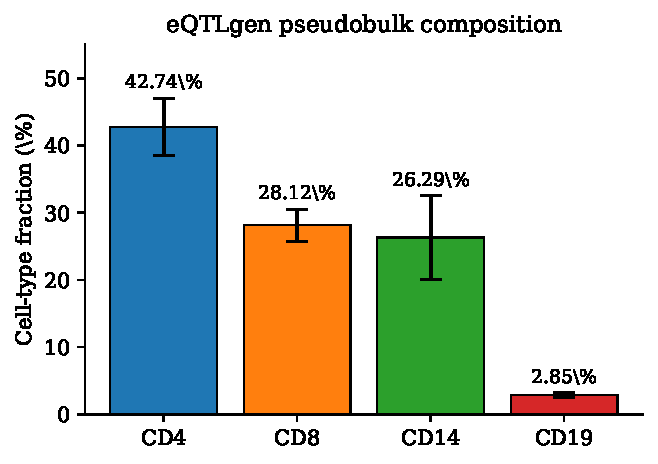
\includegraphics[width=0.6\textwidth]{figures/fig_eqtlgen_fractions.pdf}
\caption{Cell-type fractions used to generate pseudobulk samples from eQTLgen
scRNA-seq data. Means (SD): CD4 $42.74\%$ ($4.30$), CD8 $28.12\%$ ($2.40$),
CD14 $26.29\%$ ($6.21$), CD19 $2.85\%$ ($0.36$).}
\label{fig:eqtlgen_fractions}
\end{figure}
